\documentclass[specialist,
			   substylefile = spbu_report.rtx,
			   subf,href,colorlinks=true, 12pt]{disser}

\usepackage[a4paper,
			mag=1000, includefoot,
			left=3cm, right=1.5cm, top=2cm, bottom=2cm, headsep=1cm, footskip=1cm]{geometry}
\usepackage[utf8]{inputenc}
\usepackage[backend = bibtex8,sorting=none]{biblatex}
\usepackage[T2A]{fontenc}
\usepackage[english,russian]{babel}
\usepackage{amsfonts}
\usepackage{amsmath}
\usepackage{listings}
\usepackage{graphicx}
\usepackage{float}
\ifpdf\usepackage{epstopdf}\fi
% Точка с запятой в качестве разделителя между номерами цитирований
%\setcitestyle{semicolon}

\graphicspath{ {images/} }
\addbibresource{lit.bib}

% Использовать полужирное начертание для векторов
\let\vec=\mathbf

% Включать подсекции в оглавление
\setcounter{tocdepth}{2}

\makeatletter
\setlength{\@fptop}{0pt}
\makeatother

%----------------------------------------------------------------
\begin{document}

%
% Титульный лист на русском языке
%
% Название организации
\institution{%
	Санкт-Петербургский государственный университет\\
	Прикладная математика и информатика
}

\title{Отчет по учебной практике 1 (проектно-технологической) (семестр 1)}

% Тема
\topic{Использование метода SSA для анализа временных рядов на языке Python}

% Автор
\author{Козак Михаил Валерьевич}
\group{группа 21.М03-мм}

% Научный руководитель
\sa       {Голяндина Нина Эдуардовна\\%
		   Кафедра Статистического Моделирования}
\sastatus {к.\,ф.-м.\,н., доцент}

% Город и год
\city{Санкт-Петербург}
\date{2021}

\maketitle

\tableofcontents

\chapter{Введение}

Singular spectrum analysis \cite{ssa-method} – метод для анализа временных рядов, основанный на преобразовании одномерного временного ряда в многомерный, с последующим применением к нему метода главных компонент. Данный метод находит применение в различных сферах: климатология, океанология, геофизика, техника, обработка изображений, медицина, эконометрика и многие другие. \\

Для использования SSA не требуется предварительное задание модели для анализа различных произвольных рядов. Основная цель данного метода заключается в разложении ряда в сумму интерпретируемых компонент: тренд, преиодические компоненты, шум. Полученное разложение может служить основой для  прогнозирования дальнейших изменений как самого ряда, так и его отдельных составляющих.\\

В рамках данной работы были рассмотрены как написанный для языка R пакет Rssa \cite{rssa-book, rssa-doc}, так и уже существующие реализации данного метода для языка Python \cite{pyts-doc, kaggle-ssa-doc, git-kieferc-doc}, недостаток которых заключается в том, что они не обладают большой скоростью в связи с тем, что в их реализации не используются быстрые алгоритмы, которые, помимо этого, в пакете Rssa реализованы с использованием кода на языке C. По этой причине было принято решение реализовать данный метод посредством адаптации существующего модуля к языку Python. \\

Помимо адаптации модуля Rssa к языку Python также возникла необходимость в визуализации результатов, в связи с чем потребовалось прибегнуть к сторонним модулям для отображения графиков в среде Python.\\

Также одной из задач является применение полученных результатов к реальным данным: разложение временного ряда на его отдельные составляющие (шум, тренд, период) и визуализация полученного разложения.\\

\chapter{Метод SSA}

Рассмотрим временной ряд длины $N > 2$: $F = (f_0, \dots, f_{N - 1}), f_i \in \mathbb{R}$. Будем также предполагать, что ряд ненулевой: $\exists  i: f_i \neq 0$. Помимо этого, числа $0, \dots, N - 1$ можно интерпретировать не только как дискретные моменты времени, но и как некоторые метки, которые имеют линейно-упорядоченную структуру.\\

Базовый алгоритм состоит из двух дополняющих друг друга этапов: разложения и восстановления.\\

\textbf{Разложение}. Пусть $L$ – некоторое целое число \textit{(длина окна)}, $1 < L < N$. Сперва необходимо провести процедуру вложения, которая переводит исходный временной ряд в последовательность многомерных векторов. Данная процедура образует $K = N - L + 1$ \textit{векторов вложения}:

\begin{equation*}
	X_i = (f_{i - 1}, \dots, f_{i + L - 2})^\mathrm{T}, 1 \leq i \leq K,
\end{equation*}

имеющих размерность L. \\

\textit{L–траекторная матрица} ряда $F$:

\begin{equation*}
	\mathbf{X} = [X_1: \dots: X_K]
\end{equation*}

состоит из векторов вложения в качестве столбцов.\\

Следующим шагом является сингулярное разложение траекторной матрицы временного ряда.\\

Пусть $\mathbf{S} = \mathbf{XX}^\mathrm{T}$. Обозначим $\lambda_1, \dots, \lambda_L$ \textit{собственные числа} матрицы $\mathbf{S}$, взятые в неубывающем порядке: $\lambda_1 \geq \dots \geq \lambda_L \geq 0$ и $U_1, \dots, U_L$ – ортонормированную систему собственных векторов матрицы $\mathbf{S}$, соответствующих собственным числам.\\

Пусть $d = \max\{i: \lambda_i > 0\}$. Если обозначить $V_i = {X^\mathrm{T} U_i \over \sqrt{\lambda_i}}, i = 1, \dots, d$, то сингулярное разложение матрицы $\mathbf{X}$ может быть записано в следующем виде:

\begin{equation*}
	\mathbf{X} = \mathbf{X}_1 + \dots + \mathbf{X}_d,
\end{equation*}

где $\mathbf{X}_i = \sqrt{\lambda_i} U_i {V_i}^\mathrm{T}$.

\textbf{Восстановление}. На основе сингулярного разложения производится процедура группировки, которая делит все множество индексов $\{1, \dots, d\}$ на $m$ непересекающихся подмножеств $I_1, \dots, I_m$.\\

Пусть $I = \{i_1, \dots, i_p\}$. Тогда \textit{результирующая матрица} $X_I$, определяется как

\begin{equation*}
	\mathbf{X}_I = \mathbf{X}_{i_1} + \dots +  \mathbf{X}_{i_p}. 
\end{equation*}

Такие матрицы вычисляются для $I = I_1, \dots, I_m$, и разложение может быть записано в сгруппированном виде

\begin{equation*}
	\mathbf{X} = \mathbf{X}_{I_1} + \dots +  \mathbf{X}_{I_m}. 
\end{equation*}

На последнем шаге алгоритма каждая матрица сгруппированного разложения переводится в новый ряд длины $N$.\\

Пусть $\mathbf{Y} \in \mathbb{R}^{L \times K}$ – некоторая матрица с элементами $y_{ij}$. Положим $L^* = min(L, K)$, $K^* = max(L, K)$ и $N = L + K - 1$. Пусть $y^*_{ij} = y_{ij}$, если $L < K$, и $y^*_{ij} = y_{ji}$ иначе. \textit{Диагональное усреднение} переводит матрицу $\mathbf{Y}$ в ряд $g_0, \dots, g_{N - 1}$ по формуле:

\begin{equation*}
	g_k = \begin{cases}
	      	{1 \over k + 1} \sum\limits_{m = 1}^{k + 1} y^*_{m,k-m+2} &\text{для} 0 \leq k < L^* - 1,\\
	      	{1 \over L^*} \sum\limits_{m = 1}^{L^*} y^*_{m,k-m+2} &\text{для} L^* - 1 \leq k < K^*,\\
      		{1 \over N - k} \sum\limits_{m = k - K^* + 2}^{N - K^* + 1} y^*_{m,k-m+2} &\text{для} K^* \leq k < N.\\
	      		
		  \end{cases}.
\end{equation*}

Применяя диагональное усреднение к результирующим матрицам $\mathbf{X}_{I_k}$, получаем ряды $\widetilde{F}^{(k)} = (\widetilde{f}_0^{(k)}, \dots, \widetilde{f}_{N - 1}^{(k)})$, и, следовательно, исходный ряд $(f_0, \dots, f_{N - 1})$ раскладывается в сумму $m$ рядов:
	
\begin{equation*}
	f_n = \sum\limits_{k=1}^{m} \widetilde{f}_n^{(k)}.
\end{equation*}

\chapter{Пакет Rssa и его адаптация к Python}

Реализация метода SSA входит в пакет Rssa, который содержит большое количество различных инструментов для анализа и прогнозирования временных рядов и обработки изображений, а также имеет множество визуальных инструментов, полезных при выборе параметров SSA и проверки результатов. Это единственная реализация метода SSA для языка R \cite{r-doc}, доступная в CRAN, а также почти наверняка самая эффективная, во многом благодаря тому, что данный пакет реализован с использованием быстрых алгоритмов на языке C.\\

В связи с тем, что данный пакет уже обладает необходимой функциональностью и эффективностью, а также с учетом сложности переписывания данных алгоритмов под специфику языка Python \cite{py-doc}, при использовании метода SSA для данного языка программирования было принято решение взять за основу существующий пакет, обращаясь к нему с помощью интерпретатора для языка R. Для решения поставленной задачи был выбран модуль rpy2 \cite{rpy-doc}, позволяющий запускать код на языке R средставами Python и обладающий весьма гибкой функциональностью. Таким образом, задача состояла в том, чтобы адаптировать код на языке R незаметно от пользователя и с минимальным ущербом в скорости работы.\\

Данные языки во многом похожи, имеют схожие типы данных, но в то же время имеют достаточно серьезные отличия, среди которых, например, встроенная поддержка векторных вычислений в языке R, которой нет в языке Python. Для решения данной проблемы возникла необходимость в использовании пакета NumPy для Python, который позволяет работать с многомерными массивами, а также имеет эффективно реализованные математические функции для работы с ними. Благо, конвертация из NumPy в R уже была реализована в модуле rpy2, но помимо этого возникла необходимость в том, чтобы связать встроенные типы данных Python с языком R. Ниже приведен программный код, отвечающий за правила конвертации, программный код самих функций опущен.\\

\noindent
\begin{minipage}{\linewidth}
\begin{lstlisting}[language=Python, caption=Конвертация из Python в R.]
import rpy2.robjects.conversion as conversion
from rpy2.robjects.numpy2ri import converter as numpy_converter

pyRssa_converter = conversion.Converter('pyRssa converter')
pyRssa_converter.py2rpy.register(type(None), none_to_null)
pyRssa_converter.py2rpy.register(range, range_to_vec)
pyRssa_converter.py2rpy.register(py_list, list_to_vec)
pyRssa_converter.py2rpy.register(dict, dict_to_vec)
conversion_rules = default_converter + pyRssa_converter +\
                                    numpy_converter
conversion.set_conversion(conversion_rules)
\end{lstlisting}
\end{minipage}

Помимо данной проблемы возникли также сложности и с операциями между константами и векторами. В языке R для того, чтобы произвести эту операцию, существуют функции lapply и sapply, которые применяют к вектору необходимую операцию поэлементно. В Python же таких операций непосредственно в самом языке нет, в связи с чем было принято решение использовать наследование классов из языка R с дополненными необходимыми операциями. Однако же эта функциональность реализована в некоторых пакетах \cite{habr-doc} для языка Python, в связи с чем есть возможность альтернативного определения операций с векторами. В листинге 3.2 приведен пример для вещественных векторов.

\begin{lstlisting}[language=Python, caption=Наследование для FloatVector.]
class FloatVector(robjects.FloatVector):
	def __init__(self, obj):
	super().__init__(obj)
	
	def __mul__(self, other):
		if isinstance(other, float):
			return r.sapply(self, "*", other)
		elif isinstance(other, int):
			return r.sapply(self, "*", other)
	
	def __truediv__(self, other):
		if isinstance(other, float):
			return r.sapply(self, "/", other)
		elif isinstance(other, int):
			return r.sapply(self, "/", other)
	
	def __add__(self, other):
		if isinstance(other, float):
			return r.sapply(self, "+", other)
		elif isinstance(other, int):
			return r.sapply(self, "+", other)
	
	__rmul__ = __mul__
	
	__radd__ = __add__
\end{lstlisting}

Аналогичным образом возникла необходимость в адаптации непосредственно функций модуля Rssa, где достаточно было лишь указать некоторые необходимые параметры, которые автоматически транслируются из Python в R посредством модуля rpy2, для которого ранее были указаны правила конвертации типов данных. 

\begin{lstlisting}[language=Python, caption=Адаптация к модулю Rssa.]
import rpy2.robjects.packages as rpackages
r_ssa = rpackages.importr('Rssa')

def ssa(ds, L, kind):
	return r_ssa.ssa(ds, L=L, kind=kind)
\end{lstlisting}

Также необходимо было визуализировать полученные результаты, и первоначальные попытки свелись к тому, чтобы точно так же обращаться к исходным средствам языка R. Однако, в силу того, что метод для визуализации графиков в пакете Rssa был переопределен и отличается от стандартного, возникли непредвиденные сложности и пришлось прибегнуть к пакету matplotlib \cite{matplotlib-doc} для языка Python, предназначенному для визуализации графиков. 

\noindent
\begin{minipage}{\linewidth}
\begin{lstlisting}[language=Python, caption=Визуализация с помощью matplotlib.]
import matplotlib.pyplot as plt

def mplot(dt, X=None, add_residuals=False, add_original=False):
	fig, ax = plt.subplots()
	series = r.attr(dt, "series")
	if X is None:
		X = range(len(series))
	if add_original:
		ax.plot(X, series, label="Original")
	ax.plot(X, dt.rx("Trend")[0], label='Trend')
	ax.plot(X, dt.rx("Seasonality")[0], label='Seasonality')
	if add_residuals:
		ax.plot(X, r.attr(dt, "residuals"), 
                  label='Residuals')
	ax.legend()
	plt.title(label="Reconstructed series")
	plt.show()
\end{lstlisting}
\end{minipage}

\begin{figure}[htp]
	\centering
	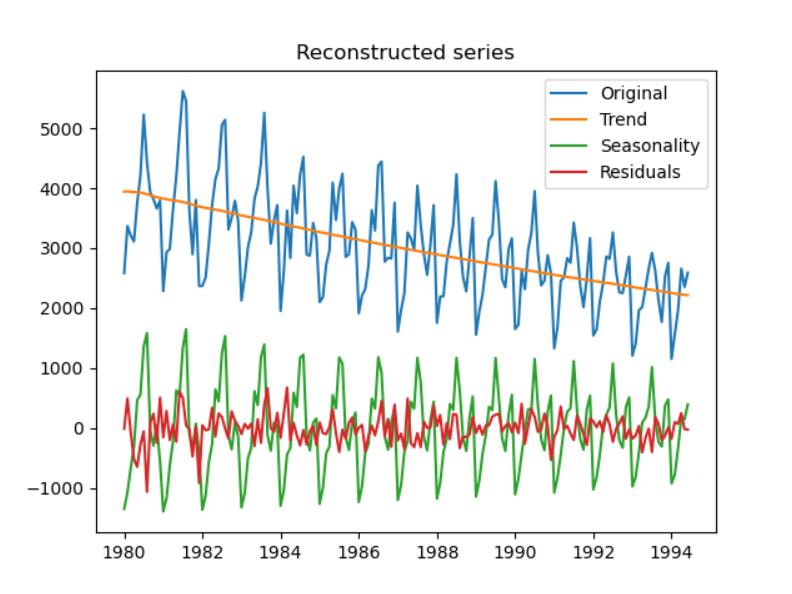
\includegraphics[width=0.65\textwidth]{py_plot_1}
	\caption{Визуализация с использованием matplotlib.}
	\label{fig:graph2}
\end{figure}



\chapter{Анализ временного ряда}

Полученный в рамках задачи по адаптации модуля Rssa к языку Python результат может быть применен к какому-либо временному ряду, однако часть функциональности, относящаяся к визуализации, в данный момент находится в процессе реализации, поэтому пример приведен на языке R. Для большей наглядности возьмем за основу модельный ряд, в котором будут присутствовать тренд, шум и сезонность. 

\begin{equation*}
	F_N = F_N^{(1)} + F_N^{(2)} + F_N^{(3)},
\end{equation*}
где $F_N^{(1)} = (f_0^{(1)}, \dots, f_{N-1}^{(1)}), f_n^{(1)} = 0.65 n$ – компонента ряда, содержащая тренд. $F_N^{(2)} = (f_0^{(2)}, \dots, f_{N-1}^{(2)}), f_n^{(2)} = \cos({2 \pi n \over 6})$ – компонента ряда, отвечающая за периодичность, а $F_N^{(3)} = (f_0^{(3)}, \dots, f_{N-1}^{(3)})$ – шум, где $f_n^{(3)}$ – независимые случайные величины, имеющие одно и то же нормальное распределение с нулевым средним и стандартным отклонением, равным $0.5$.

\begin{figure}[H]
	\centering
	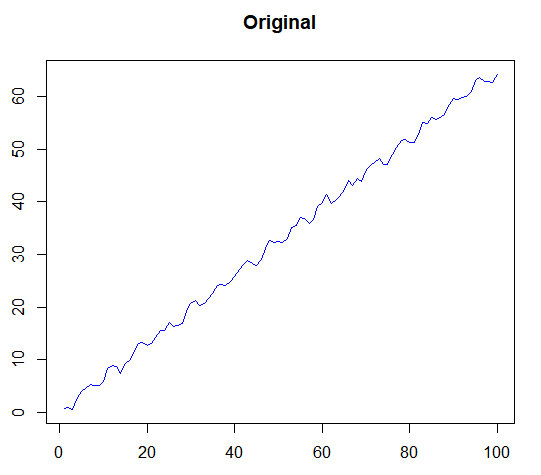
\includegraphics[width=0.5\textwidth]{r_plot_ts_orig.png}
	\caption{График исходного временного ряда.}
	\label{fig:graph3}
\end{figure}

Далее, для разложения данного ряда на тренд, шум и периодичность, необходимо задать определенную длину окна. В связи с тем, что мы будем анализировать ряд базовым методом, нет смысла брать длину окна, большую, чем половина длины ряда. Таким образом, если $N = 100$, то $L \leq 50$.\\

Для разделения временного ряда на компоненты сперва обратимся к графикам полученных с помощью метода SSA собственных векторов.

\begin{figure}[H]
	\centering
	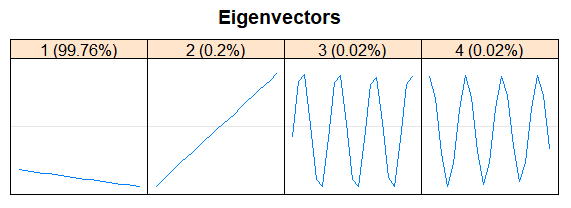
\includegraphics[width=0.5\textwidth]{r_plot_ts_eig.png}
	\caption{Собственные векторы.}
	\label{fig:graph4}
\end{figure}

В связи с тем, что в данном ряде тренд ярко выраженный, на первых позициях будет находиться большинство собственных векторов, соответствующих тренду. Таким образом, чтобы извлечь из имеющегося ряда тренд, необходимо собрать тройки, соответствующие медленно меняющимся сингулярным векторам. В данном случае, это первые два вектора.\\

Помимо этого необходимо выделить и сезонность. Третий и четвертый векторы имеют периодические колебания, в связи с чем для большей наглядности можно их сгруппировать и построить график.

\begin{figure}[H]
	\centering
	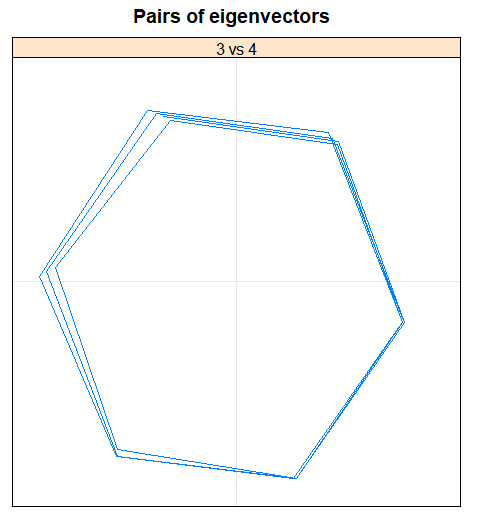
\includegraphics[width=0.25\textwidth]{r_plot_ts_pair.png}
	\caption{Двумерная диаграмма пары векторов 3 и 4.}
	\label{fig:graph5}
\end{figure}

Из данного графика достаточно хорошо видно, что период $T = 6$, так как на графике отчетливо виден шестиугольник. Это соответствует действительности, потому что в данном модельном ряде был выбран именно такой период. Далее построим реконструкцию ряда, где первая и вторая компоненты будут соответствовать тренду, а третья и четвертая – сезонности. 

\begin{figure}[H]
	\centering
	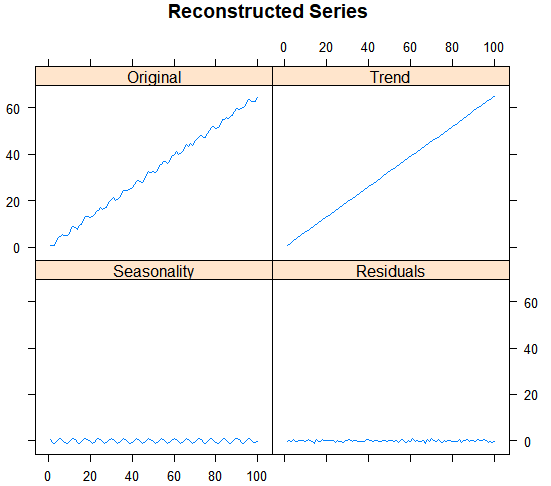
\includegraphics[width=0.6\textwidth]{r_plot_ts_rec.png}
	\caption{Реконструкция временного ряда.}
	\label{fig:graph6}
\end{figure}

С использованием средств визуализации в Python можем проверить качество получившегося разложения.

\begin{lstlisting}[language=Python, caption=Программный код для визуализации компонентов временного ряда на Python.]
import pyRssa
import numpy as np
import matplotlib.pyplot as plt

N = 100
sigma = 0.5
noise = np.array(pyRssa.r.rnorm(N)) * sigma
trend = 0.65 * pyRssa.seq(1, N)
seasonality = np.sin(2 * pyRssa.pi * pyRssa.seq(1, N) / 6)
series = seasonality + noise + trend
s_series = pyRssa.ssa(series, L=21, kind="1d-ssa")
r_series = pyRssa.reconstruct(s_series, 
    groups=pyRssa.list(Trend=range(1, 3), 
                       Seasonality=range(3, 5)))
fig, ax = plt.subplots(2, 2)
fig.suptitle("Reconstruction")
ax[0, 0].plot(pyRssa.seq(1, N), series, label="Original")
ax[0, 1].plot(pyRssa.seq(1, N), r_series.rx("Trend")[0], label='Trend')
ax[0, 1].plot(pyRssa.seq(1, N), trend, label='Original trend')
ax[0, 1].legend()
ax[1, 0].plot(pyRssa.seq(1, N), r_series.rx("Seasonality")[0], 
                                label='Seasonality')
ax[1, 0].plot(pyRssa.seq(1, N), seasonality,
                                label='Original seasonality')
ax[1, 0].legend()
ax[1, 1].plot(pyRssa.seq(1, N), pyRssa.r.attr(r_series, "residuals"),
                                label='Residuals')
ax[1, 1].plot(pyRssa.seq(1, N), noise, label='Original residuals')
ax[1, 1].legend()
plt.show()	
\end{lstlisting}

\begin{figure}[H]
	\centering
	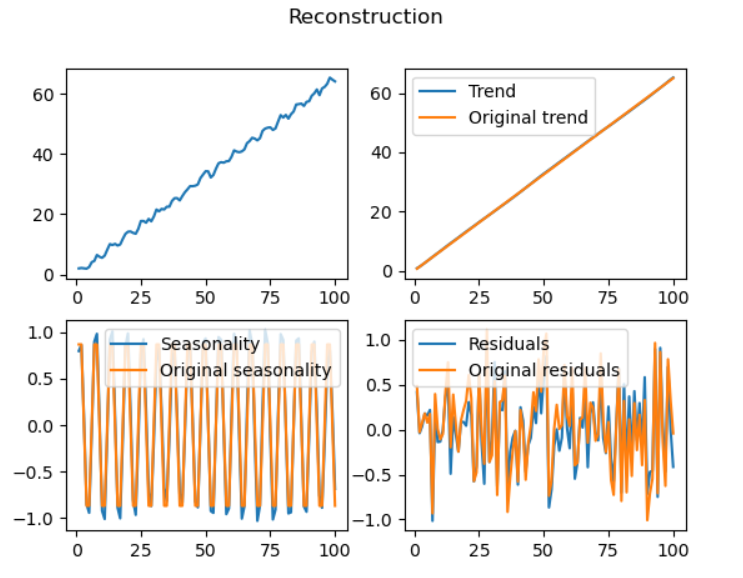
\includegraphics[width=0.6\textwidth]{py_plot_ts_rec.png}
	\caption{Реконструкция временного ряда.}
	\label{fig:graph7}
\end{figure}

Как видно из графиков, точность разложения достаточно высока, а тренд и сезонность определились практически идеально. 

\chapter{Сравнение скорости Rssa и pyRssa}

При использовании пакета Rssa в качестве основы для реализации метода SSA на языке Python одной из важнейших характеристик является скорость, а если быть точнее, то ее сохранение близкой к исходной. Далее приведен фрагменты кода на Python, а также указана скорость работы для каждого из них.

\begin{lstlisting}[language=Python, caption=Программный код для анализа скорости работы на Python.]
import pyRssa
import numpy as np
pyRssa.seed(1)
N = 71
sigma = 5
Ls = [12, 24, 36, 48, 60]
length = 24
signal_1 = 30 * np.cos(2 * pyRssa.pi * pyRssa.seq(1, N + length) / 12)
signal_2 = 30 * np.cos(2 * pyRssa.pi * pyRssa.seq(1, N + length) / 12 
                                                      + pyRssa.pi / 4)
signal = pyRssa.r.cbind(signal_1, signal_2)
R = 100
def errors(Ls):
	f1 = signal_1[:N] + pyRssa.r.rnorm(N, sd=sigma)
	f2 = signal_2[:N] + pyRssa.r.rnorm(N, sd=sigma)
	f = pyRssa.r.cbind(f1, f2)
	err_rec = pyRssa.r.numeric(5)
	err_for = pyRssa.r.numeric(5)
	for l in range(len(Ls)):
		L = Ls[l]
		s = pyRssa.ssa(f, L=L, kind="mssa")
		rec = pyRssa.reconstruct(s,groups=pyRssa.list([1,2]))
		err_rec[l] = pyRssa.mean((rec[0] - signal[:N]) ** 2)
		pred = pyRssa.vforecast(s, groups=pyRssa.list([1, 2]), 
                      direction="row", len=length, drop=True)
		err_for[l] = pyRssa.mean((pred - signal[N:]) ** 2)
	return pyRssa.list(Reconstruction=err_rec, Forecast=err_for)
res = pyRssa.replicate(R, errors, Ls)
\end{lstlisting}

\begin{table}[htp]
\centering
\begin{tabular}{ | l | l | l | l | l | l |}
	\hline
	R= & 10 & 25 & 50 & 75 & 100 \\ \hline
	R & 0.69 & 1.55 & 2.79 & 4.33 & 5.71  \\
	Python & 0.81 & 1.95 & 3.60 & 5.48 & 7.29 \\
	\hline
\end{tabular}
\caption{\label{tab:r-py-table} Сравнение скорости работы.}
\end{table}

Из таблицы видно, что пакет pyRssa уступает по скорости Rssa. На это есть логичные причины в виде автоматической конвертации из типов данных R в NumPy и наоборот, а также возможные задержки между обращением к интерпретатору языка R посредством Python.

\chapter{Заключение}

В рамках данной работы были рассмотрены уже существующие реализации метода SSA для языка Python, изучены некоторые особенности пакета Rssa, а также реализована часть методов и примеров применения данного пакета.\\

Помимо адаптации модуля Rssa к языку Python удалось применить модуль matplotlib для визуализации результатов, заменив тем самым встроенные в R средства отрисовки графиков, обращение к которым в связи с особенностями для пакета Rssa было осложнено.\\

С использованием полученных результатов, а также теории по базовому методу SSA проанализирован и разложен на отдельные компоненты модельный ряд, изучены некоторые особенности, связанные с правильным выбором параметров для метода SSA, таких как длина окна и компоненты, составляющие тренд и сезонность временного ряда.\\

С учетом текущей скорости работы модуля pyRssa по сравнению с Rssa, все еще остается необходимым продолжать работу над оптимизацией модуля, а также расширять возможности использования в SSA встроенных в Python структур данных и визуализации результатов работы.

\printbibliography
\addcontentsline{toc}{chapter}{Список литературы}

\end{document}